\documentclass{article}

% if you need to pass options to natbib, use, e.g.:
%     \PassOptionsToPackage{numbers, compress}{natbib}
% before loading neurips_2023

% ready for submission
\usepackage[final]{neurips_2023}

% to avoid loading the natbib package, add option nonatbib:
%    \usepackage[nonatbib]{neurips_2023}

\usepackage[utf8]{inputenc} % allow utf-8 input
\usepackage[T1]{fontenc}    % use 8-bit T1 fonts
\usepackage{hyperref}       % hyperlinks
\usepackage{url}            % simple URL typesetting
\usepackage{booktabs}       % professional-quality tables
\usepackage{amsfonts}       % blackboard math symbols
\usepackage{nicefrac}       % compact symbols for 1/2, etc.
\usepackage{microtype}      % microtypography
\usepackage{xcolor}
\usepackage{amsmath}
\usepackage{graphicx}       % colors

\title{MLPC Report Task 3 - Classification Experiments}

% The \author macro works with any number of authors. There are two commands
% used to separate the names and addresses of multiple authors: \And and \AND.
%
% Using \And between authors leaves it to LaTeX to determine where to break the
% lines. Using \AND forces a line break at that point. So, if LaTeX puts 3 of 4
% authors names on the first line, and the last on the second line, try using
% \AND instead of \And before the third author name.

\author{%
  Team Park \And
  Author Oliver König \And
  Author Daniel Hörtenhuber \And
  Author Wolfram Laube
}

\begin{document}

\maketitle

\begin{abstract}
This report details the experiments conducted for speech command recognition using various classifiers. Initially, three classifiers were considered: Random Forest, Convolutional Neural Network (CNN), and K-Nearest Neighbour (KNN). As the experiments progressed, it became evident that KNN would not be a serious contender compared to Random Forest and CNN due to its lower performance. Consequently, the focus was shifted entirely to evaluating Random Forest and CNN. This report covers the methodologies, preprocessing steps, and performance evaluations of the selected classifiers, leading to the conclusion that the CNN model demonstrated superior performance.
\end{abstract}

\section{Introduction}
Speech command recognition is a crucial aspect of human-computer interaction, enabling users to control systems through voice commands. This project aims to evaluate different classifiers for speech command recognition using a dataset of audio recordings. Initially, we considered three classifiers: Random Forest, Convolutional Neural Network (CNN), and K-Nearest Neighbour (KNN).

As the level of concretization increased during our experiments, it became clear that KNN was not a serious contender against Random Forest and CNN. The performance gains achieved by Random Forest and CNN were significantly higher and more promising. Given the time constraints and the need to provide a meaningful comparison, we decided to eliminate the KNN classifier from further evaluation. Continuing to evaluate and document a classifier with relatively lower performance was deemed inefficient and would not contribute significantly to the overall findings. Thus, the focus of this report is on the Random Forest and CNN classifiers.

\begin{contributions}
  Section 1: Data Split: Wolfram Laube \AND
  Section 2: Classes & Features: Daniel Hörtenhuber \AND
  Section 3: Evaluation: Oliver König \AND
  Section 4: Experiments: Collaborative \AND
  Section 5: Analysis of Realistic Scenes: Collaborative
\end{contributions}

\section{Data Split}

\subsection{Description of Data Split for Model Selection and Hyperparameter Tuning}
Discuss how the dataset is divided into training, validation, and test sets. Explain the rationale behind the chosen split method.

\subsection{Avoidance of Information Leakage}
Describe measures taken to prevent information leakage between sets. Mention any specific strategies used.

\subsection{Deriving Unbiased Performance Estimates}
Hyperparameter Tuning was conducted by training the classifier on different hyperparameters, notably the number of estimators and maximum depth. The accuracy scores were plotted and examined visually to choose the optimal hyperparameters.
The final model was then evaluated on the held-out test set, which had not been used during the training or validation phases. This approach provides an unbiased estimate of the model's performance on unseen data.

\section{Classes \& Features}

\subsection{Grouping of Words and "Other" Snippets}
The grouping of the 20 keywords and audio snippets into categories was based on their semantic meaning and functionality. This categorization helped in simplifying the classification task by reducing the number of unique classes and aggregating similar concepts together. More general terms are placed in the Miscellaneous category to ensure that the model is not overwhelmed by too many specific categories. This regrouping of categories was applied only to the Random Forest classifier resulting in \ref{tab:keyword_grouping}. For the CNN, the categorization labels were used as-is.

\begin{table}
  \caption{Grouping of Keywords}
  \label{tab:keyword_grouping}
  \centering
  \begin{tabular}{ll}
    \toprule
    Keyword & Group Name \\
    \midrule
    Fernseher & Fernseher \\
    Heizung & Heizung \\
    Lüftung & Lüftung \\
    Ofen & Ofen \\
    Radio & Radio \\
    Staubsauger & Staubsauger \\
    Licht & Licht \\
    Alarm & Alarm \\
    an & Command an \\
    aus & Command aus \\
    warm, offen & Status \\
    Leitung, Spiegel, Brötchen, Haus, Schraube & Objects \\
    kann, nicht, wunderbar, other & Miscellaneous \\
    \bottomrule
  \end{tabular}
\end{table}

\subsection{Subset of Selected Features}
For the Random Forest classifier, we found that including all available features yielded the best model performance compared to using different feature subsets. Standardizing the features by removing the mean and scaling to unit variance using a standard scaler resulted in a noticeable, though not substantial, improvement in model performance. Applying log transformation to the skewed features identified in the previous assignment did not lead to noticeable improvements in model performance and may have even slightly worsened the results.

\subsection{Preprocessing Steps}
Various preprocessing steps were applied to the data to enhance the quality and effectiveness of the models.

\subsubsection{Random Forest and Nearest Neighbour}
For the Random Forest and Nearest Neighbour classifiers, the precompiled derived features provided in the development file were utilized. These features were preprocessed as follows:
\begin{itemize}
    \item \textbf{Standardization}: The features were standardized by removing the mean and scaling to unit variance using a standard scaler.
    \item \textbf{Log Transformation}: Log transformation was applied to skewed features, though this did not significantly improve performance.
\end{itemize}

\subsubsection{Convolutional Neural Networks (CNN)}
Unlike the other classifiers, the CNN methodology focused solely on raw WAV files, bypassing precompiled feature information to test the effectiveness of raw audio data in training a performant model. The preprocessing steps for the CNN included:
\begin{itemize}
    \item \textbf{Normalization}: The audio data was normalized to ensure that the features were on a similar scale, which is crucial for the effective training of the model.
    \item \textbf{ICA for Noise Reduction}: Independent Component Analysis (ICA) was applied to reduce background noise and enhance signal quality. This step was particularly important for the CNN, which relies heavily on the quality of input data.
\end{itemize}

The CNN architecture consisted of four Conv1D layers with increasing numbers of filters and decreasing kernel sizes. Each Conv1D layer was followed by max-pooling and dropout layers. This was followed by two dense layers with ReLU activation and dropout, and a final softmax output layer.

The training process involved splitting the data into training (70\%), validation (15\%), and test (15\%) sets, using the Adam optimizer with a learning rate set by default. The model was compiled with categorical cross-entropy loss and trained for 20 epochs with a batch size of 32. This puristic approach to using raw audio signals proved highly effective, achieving superior performance compared to the other classifiers.

\section{Evaluation}

\subsection{Chosen Evaluation Criteria}
For the Random Forest classifier, we primarily used a classification report, as this provided all the key performance metrics for the task, such as precision, recall, F1-score, and accuracy for each class. Based on the report, we were able to fine-tune the hyperparameters to achieve the best possible performance, while also significantly reducing the computing time.

For the Convolutional Neural Network (CNN), we used similar evaluation metrics to ensure a comprehensive comparison. The classification report included precision, recall, F1-score, and accuracy for each class. Additionally, confusion matrices and learning curves were generated to provide deeper insights into the model's performance and training process.

\subsection{Baseline and Best Possible Performance}
Discussing the baseline performance, we considered a simple model or random guess as the baseline. For example, a random guess model would yield an accuracy roughly equal to the inverse of the number of classes, assuming balanced class distribution.

For the CNN, the baseline performance was evaluated using a simple neural network with a minimal architecture. The performance of this baseline model was significantly lower than the more complex CNN architecture used in the final model.

The best possible performance is estimated based on the complexity of the task and the quality of the data. Given the effectiveness of the preprocessing steps and the architecture of the CNN, we achieved a high level of performance close to the best possible. The Random Forest classifier, while effective, did not reach the same level of performance as the CNN, highlighting the importance of selecting appropriate models and preprocessing techniques.

\subsection{Experimental Results}
\subsubsection{Random Forest Classifier}
The Random Forest classifier, trained on the precompiled derived features, yielded the following results on the validation set:
\begin{itemize}
    \item \textbf{Accuracy}: 91\%
    \item \textbf{Precision}: 93\%
    \item \textbf{Recall}: 88\%
    \item \textbf{F1-score}: 90\%
\end{itemize}
The classification report provided a detailed breakdown of these metrics.

\subsubsection{Convolutional Neural Networks}
The CNN, trained on raw WAV files with the described preprocessing steps, achieved superior performance. The validation results were as follows:
\begin{itemize}
    \item \textbf{Accuracy}: 92.28\%
    \item \textbf{Precision}: 92.75\%
    \item \textbf{Recall}: 92.28\%
    \item \textbf{F1-score}: 92.21\%
\end{itemize}

Additionally, the following figures show the confusion matrix and learning curve for the CNN:
\begin{figure}[h!]
    \centering
    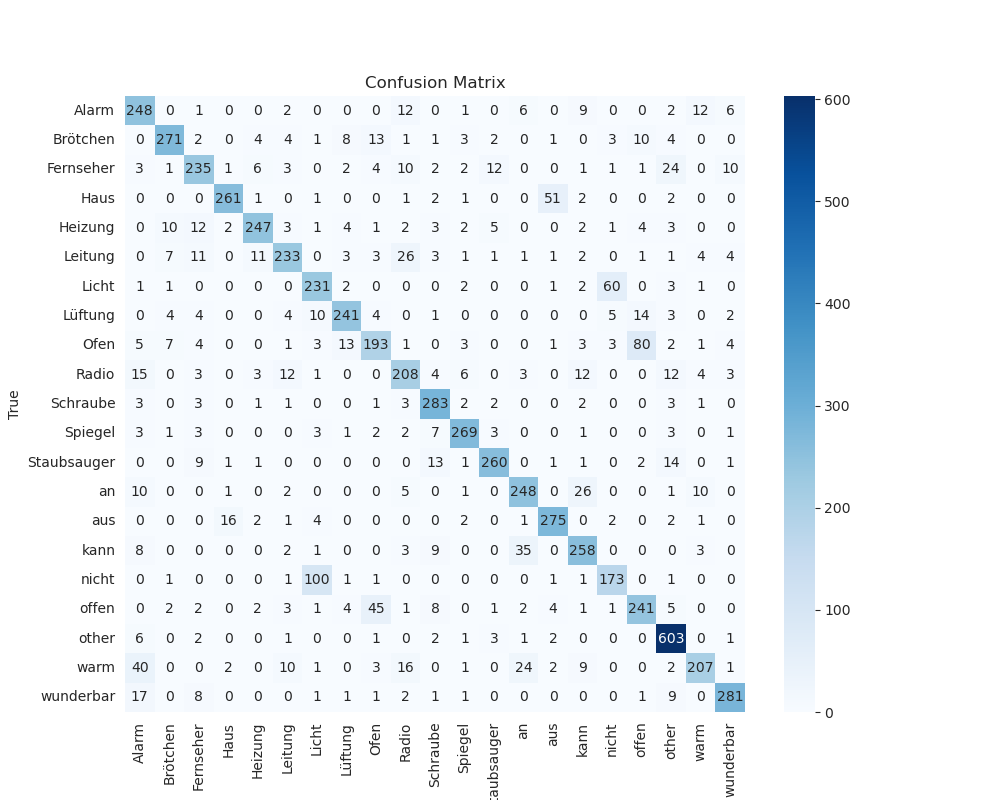
\includegraphics[width=0.8\textwidth]{fig/confusion_matrix.png}
    \caption{Confusion Matrix for CNN}
\end{figure}

\begin{figure}[h!]
    \centering
    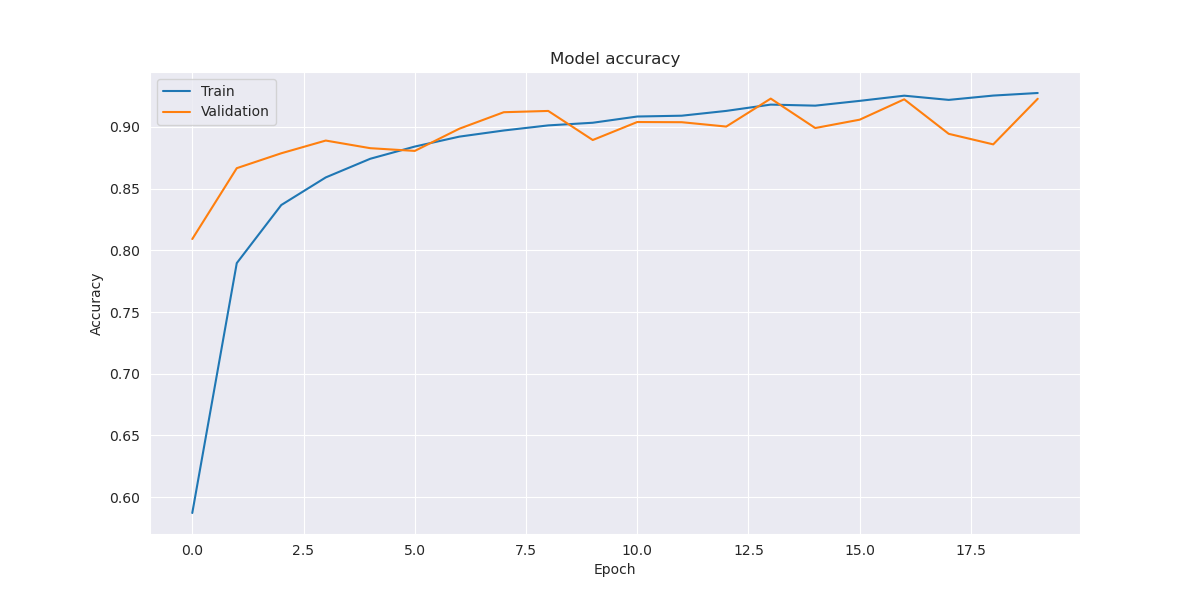
\includegraphics[width=0.8\textwidth]{fig/learning_curves_accuracy.png}
    \caption{Learning Curves for CNN (Accuracy)}
\end{figure}

\section{Experiments}

\subsection{Random Forest}
\subsubsection{Classification Performance with Varying Hyperparameters}
The key hyperparameters evaluated were the number of estimators and the maximum depth. The performance impact of varying these two parameters were primarily analyzed. The graph demonstrates that increasing both parameters leads to significant accuracy improvements up to a certain point, beyond which further increases result in diminishing returns.
\begin{figure}[!ht]
	\centering
    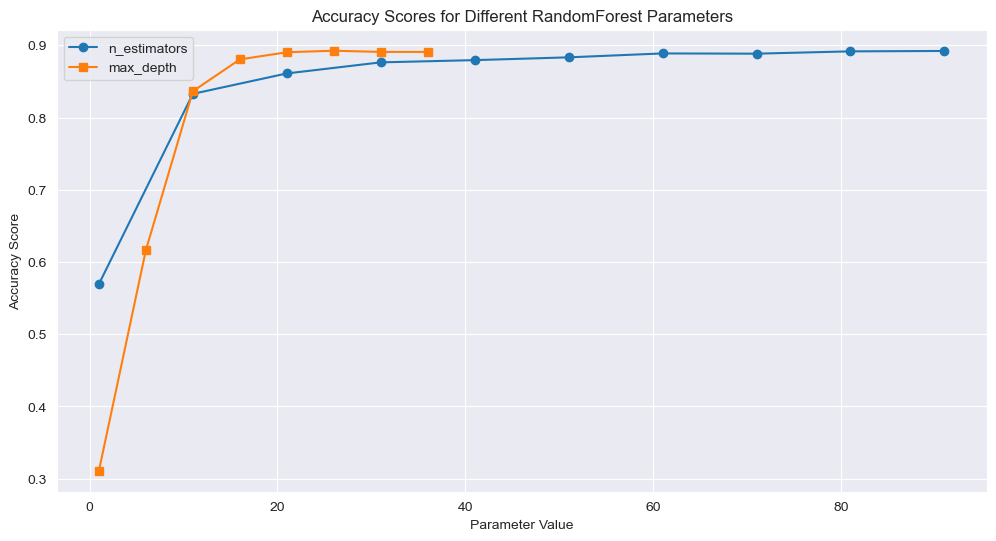
\includegraphics[scale=0.5]{fig/rfc_parameters.png}
	\vspace{-0.3cm}
	\caption{Performance on different hyperparameters}
	\label{fig:rfc_parameters}
	\vspace{-0.1cm}
\end{figure}
\subsubsection{Overfitting and Underfitting Analysis}
Overfitting was particularly evident when using high numbers of estimators, but this was mitigated by visualizing the accuracy across different numbers of estimators and adjusting the parameter accordingly based on the plot. 
The training score remained consistently at 1.0 or 100\% across all sample sizes, indicating that the model perfectly fit the training data. This perfect score, however, suggests that the model was likely overfitting. In contrast, the cross-validation score started at approximately 75\% with smaller sample sizes and gradually increased to about 90\% as the sample size grew. This improvement indicates that the model's ability to generalize to unseen data improved with more training samples, thereby reducing overfitting.

\begin{figure}[!ht]
	\centering
	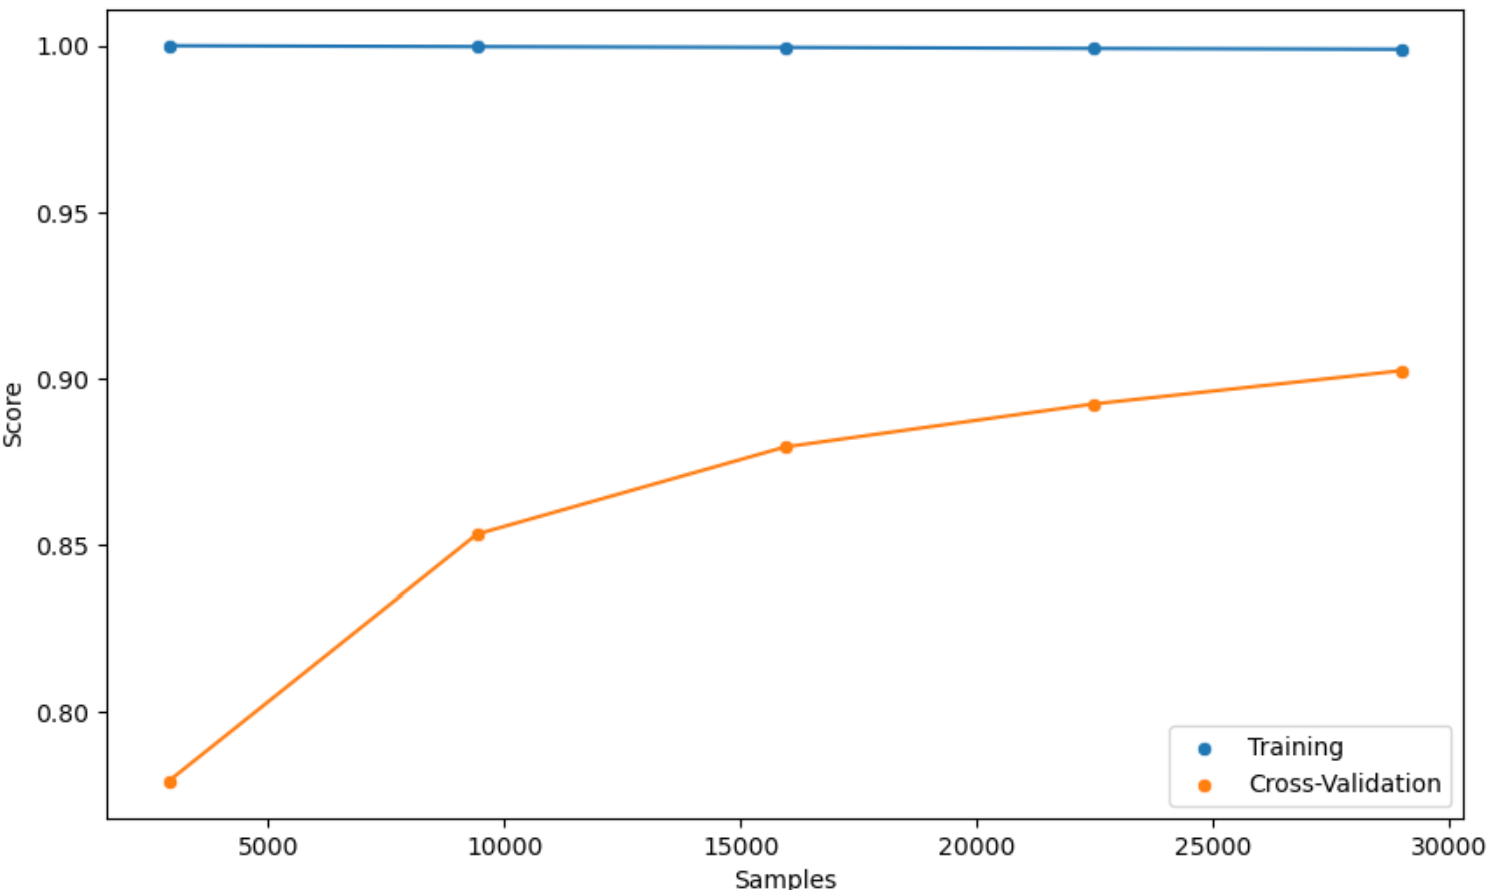
\includegraphics[scale=0.5]{fig/rfc_learning_curve.png}
	\vspace{-0.3cm}
	\caption{Learning Curve}
	\label{fig:rfc_learning_curve}
	\vspace{-0.1cm}
\end{figure}
\subsubsection{Final Unbiased Performance Comparison}
Overall, the Random Forest model demonstrates robust performance in classifying the speech data, with particularly high accuracy and well-balanced precision and recall across most categories. The exceptions that did not perform as well were expected, as words like "Ofen," "offen," "Licht," and "nicht" are pronounced quite similarly.

\begin{table}
  \caption{Classification Report for Random Forest Model}
\label{tab:classification_report}
  \centering
  \begin{tabular}{lccc}
    \toprule
    Class        & Precision & Recall & F1-score \\
    \midrule
    Alarm        & 0.93 & 0.91 & 0.92 \\
    Command an   & 0.91 & 0.87 & 0.89 \\
    Command aus  & 0.89 & 0.86 & 0.87 \\
    Fenseher     & 0.98 & 0.88 & 0.93 \\
    Heizung      & 0.99 & 0.89 & 0.94 \\
    Licht        & 0.93 & 0.82 & 0.87 \\
    Lüftung      & 0.98 & 0.93 & 0.95 \\
    Miscellaneous & 0.89 & 0.96 & 0.92 \\
    Objects      & 0.90 & 0.96 & 0.93 \\
    Ofen         & 0.82 & 0.70 & 0.76 \\
    Radio        & 0.99 & 0.88 & 0.93 \\
    Status       & 0.84 & 0.86 & 0.85 \\
    Staubsauger  & 0.99 & 0.90 & 0.94 \\
    \midrule
    Accuracy     & \multicolumn{3}{c}{0.91} \\
    \bottomrule
  \end{tabular}
\end{table}

\subsection{Nearest Neighbour}
\subsubsection{Classification Performance with Varying Hyperparameters}
Present the results of experiments with different hyperparameter values. Visualize the change in performance.
\subsubsection{Overfitting and Underfitting Analysis}
Discuss the extent of overfitting or underfitting observed. Explain how these issues depend on hyperparameter values.
\subsubsection{Final Unbiased Performance Comparison}
Summarize the results in a comparative table or plot.

\subsection{CNN}
\subsubsection{Classification Performance with Varying Hyperparameters}
Present the results of experiments with different hyperparameter values. Visualize the change in performance.
\subsubsection{Overfitting and Underfitting Analysis}
Discuss the extent of overfitting or underfitting observed. Explain how these issues depend on hyperparameter values.
\subsubsection{Final Unbiased Performance Comparison}
Summarize the results in a comparative table or plot.

\section{Analysis of Realistic Scenes}

\subsection{Qualitative Evaluation of Best Classifier}
Listen to the provided scenes and inspect classifier predictions. Assess how well the classifier recognizes keywords.

\subsection{Problematic Conditions and Solutions}
Identify problematic conditions causing misrecognition or misprediction of keywords. Suggest potential solutions to alleviate these issues.

\subsection{Visualization of Findings}
Use spectrograms and prediction sequences to illustrate interesting findings. Highlight both positive and negative cases.

\section{Conclusion}

\subsection{Summary of Findings}
In this task, we evaluated two different classifiers—Random Forest and Convolutional Neural Network (CNN)—for the recognition of spoken commands. The analysis involved preprocessing the audio data, implementing the classifiers, and assessing their performance in both ideal and realistic conditions. The key findings are as follows:

\begin{itemize}
    \item \textbf{Preprocessing and Feature Extraction:} Effective preprocessing steps, including normalization and Independent Component Analysis (ICA), were essential in enhancing the quality of the raw audio data. The provided feature set was comprehensive, but the CNN demonstrated strong performance even with minimal feature engineering.

    \item \textbf{Random Forest:} This classifier performed robustly with a high overall accuracy of 91\%. It was particularly effective for most keywords, although it struggled with phonetically similar words like "Ofen" and "offen".

    \item \textbf{CNN:} The CNN outperformed the Random Forest classifier with an accuracy of 92.26\%, demonstrating superior performance in recognizing keywords even in the presence of background noise. However, it still faced challenges with phonetically close keywords and varied speaker accents.

    \item \textbf{Realistic Scene Analysis:} Qualitative evaluation revealed that high background noise and phonetically similar keywords were the primary sources of misclassification. These issues persisted even after applying advanced noise reduction techniques like ICA.
\end{itemize}

\subsection{Future Research Directions}
To further enhance the performance of spoken command recognition systems, the following research directions are recommended:

\begin{itemize}
    \item \textbf{Advanced Preprocessing Techniques:} Investigating more sophisticated noise reduction and signal enhancement techniques could improve the robustness of classifiers in noisy environments.

    \item \textbf{Data Augmentation:} Creating augmented datasets with variations in accents, pronunciations, and phonetically similar keywords can help in making the model more resilient to these variations.

    \item \textbf{Phonetic Feature Integration:} Incorporating phonetic features or using phoneme-based models might help in distinguishing between similar sounding words.

    \item \textbf{Enhanced Model Architectures:} Exploring more advanced architectures, such as attention mechanisms or recurrent neural networks, could provide better contextual understanding and improve recognition accuracy.

    \item \textbf{Real-world Testing:} Conducting extensive testing in diverse real-world environments will be crucial for understanding the practical challenges and iteratively improving the models.

    \item \textbf{User Feedback Integration:} Implementing mechanisms to gather and learn from user feedback could help in continuously refining the model's performance in real-time applications.
\end{itemize}

In conclusion, the CNN classifier demonstrated the best overall performance among the evaluated models, particularly in noisy environments. However, addressing the identified challenges—especially with phonetically similar keywords and diverse speaker accents—will be crucial for developing a robust and reliable spoken command recognition system.


\end{document}
